\documentclass[a4paper]{article}
%\usepackage[singlespacing]{setspace}
\usepackage[onehalfspacing]{setspace}
%\usepackage[doublespacing]{setspace}
\usepackage{geometry} % Required for adjusting page dimensions and margins
\usepackage{amsmath,amsfonts,stmaryrd,amssymb,mathtools,dsfont} % Math packages
\usepackage{tabularx}
\usepackage{colortbl}
\usepackage{listings}
\usepackage{amsmath}
\usepackage{amssymb}
\usepackage{amsthm}
\usepackage{subcaption}
\usepackage{float}
\usepackage[table,xcdraw]{xcolor}
\usepackage{tikz-qtree}
\usepackage{forest}
\usepackage{changepage,titlesec,fancyhdr} % For styling Header and Titles
\pagestyle{fancy}

\usepackage{enumerate} % Custom item numbers for enumerations

\usepackage[ruled]{algorithm2e} % Algorithms

\usepackage[framemethod=tikz]{mdframed} % Allows defining custom boxed/framed environments

\usepackage{listings} % File listings, with syntax highlighting
\lstset{
	basicstyle=\ttfamily, % Typeset listings in monospace font
}

\usepackage[ddmmyyyy]{datetime}


\geometry{
	paper=a4paper, % Paper size, change to letterpaper for US letter size
	top=2.5cm, % Top margin
	bottom=3cm, % Bottom margin
	left=2.5cm, % Left margin
	right=2.5cm, % Right margin
	headheight=25pt, % Header height
	footskip=1.5cm, % Space from the bottom margin to the baseline of the footer
	headsep=1cm, % Space from the top margin to the baseline of the header
	%showframe, % Uncomment to show how the type block is set on the page
}
\lhead{Stochastik für die Informatik\\Wintersemester 2024/2025}
\chead{\bfseries{Übungsblatt 2}\\}
\rhead{Lienkamp, 8128180\\Werner, 7987847}

\begin{document}

\setcounter{section}{2} % Setzt den Section-Zähler auf 2
\subsection{Bedingte Wahrscheinlichkeiten}
Im U-Bahnhof Bockenheimer Warte beobachten wir einen Zug der U-Bahn-Linie U4, einen Zug der U6 und einen Zug der U7. Die U4 kommt mit Wahrscheinlichkeit 8/10 pünktlich, die U6 mit Wahrscheinlichkeit 6/10 und die U7 mit Wahrscheinlichkeit 5/10, dabei ist jeder Zug pünktlich unabhängig von allen anderen.\\
Falls genau zwei von den drei Zügen pünktlich waren, was ist wahrscheinlicher: die U7 war pünktlich, oder die U7 war nicht pünktlich?\\\\

\begin{center}
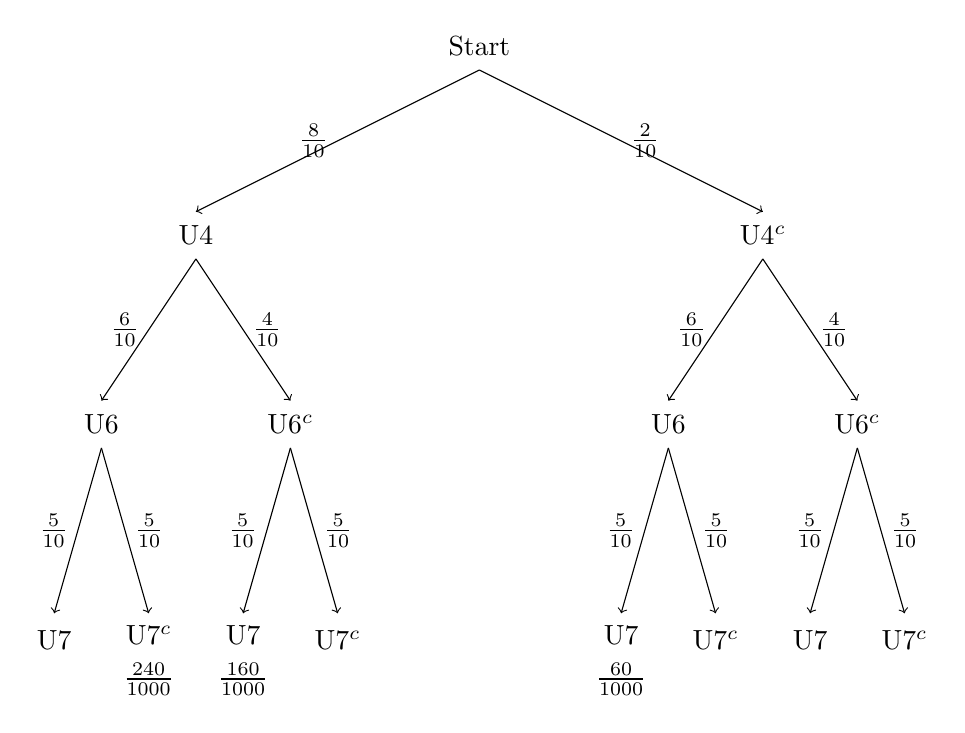
\begin{tikzpicture}[scale=1.2, every node/.style={align=center}]

    % Draw the root
    \node at (0,0) {Start};

    % First level
    \node at (-3,-2) {U4};
    \node at (3,-2) {U4$^c$};

    % Second level
    \node at (-4,-4) {U6};
    \node at (-2,-4) {U6$^c$};

    \node at (2,-4) {U6};
    \node at (4,-4) {U6$^c$};

    % Third level for W1 and S1
    \node at (-4.5,-6.5) {U7 \\};
    \node at (-3.5,-6.5) {U7$^c$ \\ \(\frac{240}{1000}\)};
    
    \node at (-2.5,-6.5) {U7 \\ \(\frac{160}{1000}\)};
    \node at (-1.5,-6.5) {U7$^c$ \\};

    % Third level for S1
    \node at (1.5,-6.5) {U7 \\ \(\frac{60}{1000}\)};
    \node at (2.5,-6.5) {U7$^c$ \\};

    \node at (3.5,-6.5) {U7 \\};
    \node at (4.5,-6.5) {U7$^c$ \\};

    % Draw the branches with probabilities
    \draw[->] (0,-0.25) -- (-3,-1.75) node[midway, left] {\(\frac{8}{10}\)};
    \draw[->] (0,-0.25) -- (3,-1.75) node[midway, right] {\(\frac{2}{10}\)};
    
    \draw[->] (-3,-2.25) -- (-4,-3.75) node[midway, left] {\(\frac{6}{10}\)};
    \draw[->] (-3,-2.25) -- (-2,-3.75) node[midway, right] {\(\frac{4}{10}\)};
    
    \draw[->] (3,-2.25) -- (2,-3.75) node[midway, left] {\(\frac{6}{10}\)};
    \draw[->] (3,-2.25) -- (4,-3.75) node[midway, right] {\(\frac{4}{10}\)};
    
    % Draw branches for W1
    \draw[->] (-4,-4.25) -- (-4.5,-6) node[midway, left] {\(\frac{5}{10}\)};
    \draw[->] (-4,-4.25) -- (-3.5,-6) node[midway, right] {\(\frac{5}{10}\)};
    
    % Draw branches for S1
    \draw[->] (-2,-4.25) -- (-2.5,-6) node[midway, left] {\(\frac{5}{10}\)};
    \draw[->] (-2,-4.25) -- (-1.5,-6) node[midway, right] {\(\frac{5}{10}\)};

    % Draw branches for U2
    \draw[->] (2,-4.25) -- (1.5,-6) node[midway, left] {\(\frac{5}{10}\)};
    \draw[->] (2,-4.25) -- (2.5,-6) node[midway, right] {\(\frac{5}{10}\)};
    
    \draw[->] (4,-4.25) -- (3.5,-6) node[midway, left] {\(\frac{5}{10}\)};
    \draw[->] (4,-4.25) -- (4.5,-6) node[midway, right] {\(\frac{5}{10}\)};

\end{tikzpicture}
\end{center}

\noindent Wir rechnen nur die Wahrscheinlichkeiten aus, die für uns relevant sind, also die Wege im Baum, bei
denen genau zwei U-Bahnen pünktlich kommen.\\\\
Ob eine Bahn pünktlich oder nicht ist, wird als $P$/$P^c$ definiert.\\\\
\(\mathbb{P}(P\cap P \cap P^c)= \{\{U4 \cap U6 \cap U7^c\},\{U4 \cap U6^c \cap U7\}, \{U4^c \cap U6 \cap U7\}\}\\
\mathbb{P}(P\cap P \cap P^c) = U4 \cap U6 \cap U7^c + U4 \cap U6^c \cap U7\ + U4^c \cap U6 \cap U7\\
\hspace*{0.5cm}\Rightarrow \frac{8}{10}\cdot\frac{6}{10}\cdot \frac{5}{10}+ \frac{8}{10}\cdot \frac{4}{10}\cdot \frac{5}{10} + \frac{2}{10}\cdot \frac{6}{10} \cdot \frac{5}{10}= \frac{240}{1000}+ \frac{160}{1000} + \frac{6}{10}= \frac{460}{1000}\\\\
\mathbb{P}(U7\vert P\cap P \cap P^c) = \{\{U4 \cap U6^c \cap U7\}, \{U4^c \cap U6 \cap U7\}\}\\
\textcolor{gray}{ \text{NR: }\mathbb{P}(P \cap P \cap U7)=\frac{8}{10}\cdot \frac{4}{10}\cdot \frac{5}{10} + \frac{2}{10}\cdot \frac{6}{10} \cdot \frac{5}{10}= \frac{160}{1000}+ \frac{60}{1000}= \frac{220}{1000}}\\
\mathbb{P}(U7\vert P\cap P \cap P^c)= \frac{P \cap P \cap U7}{P\cap P \cap P^c} = \frac{220/1000}{460/1000}=\frac{220}{460}\\
\Rightarrow \mathbb{P}(U7^c\vert P\cap P \cap P^c)= 1-\frac{220}{460}=\frac{240}{460}>\frac{220}{460}\)\\\\
Die Wahrscheinlichkeit ist größer, dass die U7 unpünktlich ist, wenn genau 2 Bahnen pünktlich kommen.
\clearpage
\subsection{}
In einer Stadt gibt es genau 40 blaue und 160 grüne Taxis. Bei einem nächtlichen Verkehrsunfall eines unbekannten Taxis mit Fahrerflucht geben zwei Zeugen unabhängig voneinander an, ein blaues Taxi gesehen zu haben. Tests ergeben, dass der erste Zeuge die Farbe eines Taxis in der Nacht mit einer Wahrscheinlichkeit von 80\% richtig bestimmt. Der zweite Zeuge erkennt ein blaues Taxi als blau mit einer Wahrscheinlichkeit von 90\% und ein grünes als grün mit 70 \%-iger Wahrscheinlichkeit. Mit welcher Wahrscheinlichkeit ist das unbekannte Taxi blau.\\
\textit{Hinweis: Sie dürfen annehmen, dass die beiden Zeugenaussagen unabhängig sind bedingt auf das Ereignis, dass das unbekannte Taxi blau bzw. grün ist.}\\\\

\begin{center}
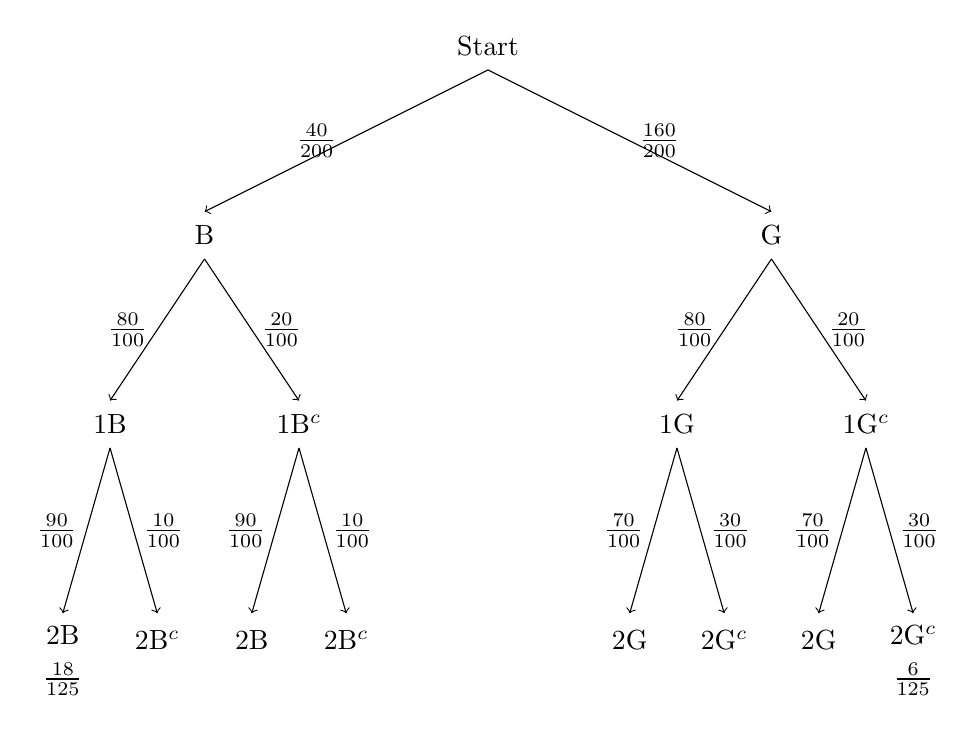
\begin{tikzpicture}[scale=1.2, every node/.style={align=center}]

    % Draw the root
    \node at (0,0) {Start};

    % First level
    \node at (-3,-2) {B};
    \node at (3,-2) {G};

    % Second level
    \node at (-4,-4) {1B};
    \node at (-2,-4) {1B$^c$};

    \node at (2,-4) {1G};
    \node at (4,-4) {1G$^c$};

    % Third level for W1 and S1
    \node at (-4.5,-6.5) {2B \\ \(\frac{18}{125}\)};
    \node at (-3.5,-6.5) {2B$^c$ \\};
    
    \node at (-2.5,-6.5) {2B \\};
    \node at (-1.5,-6.5) {2B$^c$ \\};

    % Third level for S1
    \node at (1.5,-6.5) {2G \\};
    \node at (2.5,-6.5) {2G$^c$ \\};

    \node at (3.5,-6.5) {2G \\};
    \node at (4.5,-6.5) {2G$^c$ \\\(\frac{6}{125}\)};

    % Draw the branches with probabilities
    \draw[->] (0,-0.25) -- (-3,-1.75) node[midway, left] {\(\frac{40}{200}\)};
    \draw[->] (0,-0.25) -- (3,-1.75) node[midway, right] {\(\frac{160}{200}\)};
    
    \draw[->] (-3,-2.25) -- (-4,-3.75) node[midway, left] {\(\frac{80}{100}\)};
    \draw[->] (-3,-2.25) -- (-2,-3.75) node[midway, right] {\(\frac{20}{100}\)};
    
    \draw[->] (3,-2.25) -- (2,-3.75) node[midway, left] {\(\frac{80}{100}\)};
    \draw[->] (3,-2.25) -- (4,-3.75) node[midway, right] {\(\frac{20}{100}\)};
    
    % Draw branches for W1
    \draw[->] (-4,-4.25) -- (-4.5,-6) node[midway, left] {\(\frac{90}{100}\)};
    \draw[->] (-4,-4.25) -- (-3.5,-6) node[midway, right] {\(\frac{10}{100}\)};
    
    % Draw branches for S1
    \draw[->] (-2,-4.25) -- (-2.5,-6) node[midway, left] {\(\frac{90}{100}\)};
    \draw[->] (-2,-4.25) -- (-1.5,-6) node[midway, right] {\(\frac{10}{100}\)};

    % Draw branches for U2
    \draw[->] (2,-4.25) -- (1.5,-6) node[midway, left] {\(\frac{70}{100}\)};
    \draw[->] (2,-4.25) -- (2.5,-6) node[midway, right] {\(\frac{30}{100}\)};
    
    \draw[->] (4,-4.25) -- (3.5,-6) node[midway, left] {\(\frac{70}{100}\)};
    \draw[->] (4,-4.25) -- (4.5,-6) node[midway, right] {\(\frac{30}{100}\)};

\end{tikzpicture}
\end{center}
Wir definieren:\\
- $B$/$G$ Das Taxi ist tatsächlich blau/grün\\
- \textit{1B}/\textit{1B}$^c$ Einer der beiden Zeugen sagt, das Taxi \textit{ist}/\textit{ist nicht} blau, wenn das Taxi blau war.\\
- \textit{1G}/\textit{1G}$^c$ Einer der beiden Zeugen sagt, das Taxis \textit{ist}/\textit{ist nicht} grün, wenn das Taxi 
grün war.\\
- Analog gilt das gleiche für den anderen Zeugen bei \textit{2B}/\textit{2B}$^c$ und \textit{2G}/\textit{2G}$^c$
\\\\
Wir berechnen die Wahrscheinlichkeit, dass das Taxi blau ist ($A$) unter der Bedingung, dass beide Zeugen sagen, dass das Taxi blau ist ($B$):\\
%\(\mathbb{P}(B)=\{\{B, 1B, 2B\}, \{G, 1B, 2B\}\}\\
\(\textcolor{gray}{\mathbb{P}(B)= \frac{2}{10}\cdot \frac{8}{10} \cdot \frac{9}{10} + \frac{8}{10}\cdot \frac{2}{10}\cdot \frac{3}{10}= \frac{144}{1000}+\frac{48}{1000}=\frac{192}{1000}}\\
\textcolor{gray}{\mathbb{P}(A \cap B ) = \frac{2}{10}\cdot \frac{8}{10} \cdot \frac{9}{10} = \frac{144}{1000}}\\
\mathbb{P}(A \vert B)= \frac{\mathbb{P}(A \cap B)}{\mathbb{P}(B)}\Rightarrow \frac{144/1000}{192/1000}=\frac{3}{4}\)\\
Die Wahrscheinlichkeit, dass das Taxi blau ist, ist $\frac{3}{4}$.
\clearpage
\subsection{}
An einem zufällig ausgewählten Tag ist Ava mit Wahrscheinlichkeit 7\% krank und Ben mit Wahrscheinlichkeit 5\%. Da beide Geschwister sind, passiert das nicht notwendigerweise unabhängig voneinander. Außerdem sind mit 96 \%-iger Wahrscheinlichkeit, entweder beide gesund oder beide krank. Bestimmen Sie die Wahrscheinlichkeit, dass Ava krank ist, unter der Bedingung, dass Ben krank ist.\\\\
Wir benutzen die Vier-Felder-Tafel um das Problem zu lösen:\\\\
\begin{tabular}{c|c|c|c}
     & $A$ & $A^c$ \\
    \hline
    & & & \\
    $B$ & $c=\frac{4}{100}$ & $d=\frac{1}{100}$ & $\frac{5}{100}$\\
    & & & \\
    \hline
    & & & \\
    $B^c$ & $e=\frac{3}{100}$ & $f=\frac{92}{100}$ & $\frac{95}{100}$\\
    & & & \\
    \hline
    & $\frac{7}{100}$ & $\frac{93}{100}$ & 1
\end{tabular}\\\\
Dafür stellen wir zunächst ein Gleichungssystem auf:\\
i) \space\space\(c+d=\frac{5}{100}\)\\
ii) \space\(c+e=\frac{7}{100}\)\\
iii) \(d+f=\frac{93}{100}\)\\
iv) \(e+f=\frac{95}{100}\)\\
v) \space \(c+f=\frac{96}{100}\)\\\\
Danach formen wir die aufgestellten Formeln um, um die fehlenden Felder einzufüllen:\\
i) $c= \frac{5}{100}-d$\\
iii) $f = \frac{93}{100}-d$\\
i) und iii) in v) $\frac{5}{100}-d + \frac{93}{100}-d = \frac{96}{100} \Rightarrow \frac{98}{100}-2d = \frac{96}{100} \Rightarrow d=\frac{1}{100}$\\
d in i) $c = \frac{5}{100}-\frac{1}{100}=\frac{4}{100}$\\
c in ii) $\frac{4}{100}+e=\frac{7}{100}\Rightarrow e=\frac{6}{100}$\\
e in iv) $\frac{6}{100}+f=\frac{95}{100}\Rightarrow f = \frac{92}{100}$\\\\
\textcolor{gray}{NR: \(\mathbb{P}(A \cap B)=\frac{4}{100}\) \& \(\mathbb{P}(B)= \frac{5}{100}\)}\\
$\mathbb{P}(A \vert B) = \frac{\mathbb{P}(A \cap B)}{\mathbb{P}(B)}= \frac{4/100}{5/100}=\frac{4}{5}$\\\\
Die Wahrscheinlichkeit, dass Ava krank ist unter der Bedingung, dass Ben auch krank ist liegt bei 80\%.
\clearpage
\subsection{Unabhängigkeit}
Es sei A das Ereignis, dass eine Familie Kinder beiderlei Geschlechts hat sowie B das Ereignis, dass eine Familie höchstens einen Sohn hat. Sie dürfen annehmen, dass jedes Kind, unabhängig von den anderen Kindern, mit Wahrscheinlichkeit 0.5 ein Mädchen ist.\\
Geben Sie jeweils einen Wahrscheinlichkeitsraum an und definieren Sie Ihre Ereignisse entsprechend.\\\\
(a) Unter der Voraussetzung, dass eine Familie genau drei Kinder hat, zeigen Sie, dass A und B unabhängige Ereignisse sind.
\begin{center}
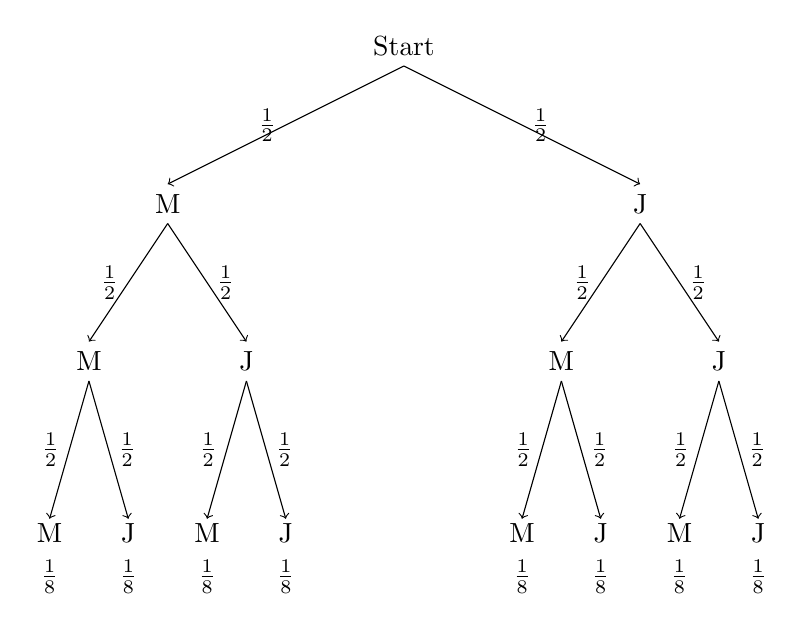
\begin{tikzpicture}[scale=1, every node/.style={align=center}]

    % Draw the root
    \node at (0,0) {Start};

    % First level
    \node at (-3,-2) {M};
    \node at (3,-2) {J};

    % Second level
    \node at (-4,-4) {M};
    \node at (-2,-4) {J};

    \node at (2,-4) {M};
    \node at (4,-4) {J};

    % Third level for W1 and S1
    \node at (-4.5,-6.5) {M \\ \(\frac{1}{8}\)};
    \node at (-3.5,-6.5) {J \\ \(\frac{1}{8}\)};
    
    \node at (-2.5,-6.5) {M \\ \(\frac{1}{8}\)};
    \node at (-1.5,-6.5) {J \\ \(\frac{1}{8}\)};

    % Third level for S1
    \node at (1.5,-6.5) {M \\ \(\frac{1}{8}\)};
    \node at (2.5,-6.5) {J \\ \(\frac{1}{8}\)};

    \node at (3.5,-6.5) {M \\ \(\frac{1}{8}\)};
    \node at (4.5,-6.5) {J \\ \(\frac{1}{8}\)};

    % Draw the branches with probabilities
    \draw[->] (0,-0.25) -- (-3,-1.75) node[midway, left] {\(\frac{1}{2}\)};
    \draw[->] (0,-0.25) -- (3,-1.75) node[midway, right] {\(\frac{1}{2}\)};
    
    \draw[->] (-3,-2.25) -- (-4,-3.75) node[midway, left] {\(\frac{1}{2}\)};
    \draw[->] (-3,-2.25) -- (-2,-3.75) node[midway, right] {\(\frac{1}{2}\)};
    
    \draw[->] (3,-2.25) -- (2,-3.75) node[midway, left] {\(\frac{1}{2}\)};
    \draw[->] (3,-2.25) -- (4,-3.75) node[midway, right] {\(\frac{1}{2}\)};
    
    % Draw branches for W1
    \draw[->] (-4,-4.25) -- (-4.5,-6) node[midway, left] {\(\frac{1}{2}\)};
    \draw[->] (-4,-4.25) -- (-3.5,-6) node[midway, right] {\(\frac{1}{2}\)};
    
    % Draw branches for S1
    \draw[->] (-2,-4.25) -- (-2.5,-6) node[midway, left] {\(\frac{1}{2}\)};
    \draw[->] (-2,-4.25) -- (-1.5,-6) node[midway, right] {\(\frac{1}{2}\)};

    % Draw branches for U2
    \draw[->] (2,-4.25) -- (1.5,-6) node[midway, left] {\(\frac{1}{2}\)};
    \draw[->] (2,-4.25) -- (2.5,-6) node[midway, right] {\(\frac{1}{2}\)};
    
    \draw[->] (4,-4.25) -- (3.5,-6) node[midway, left] {\(\frac{1}{2}\)};
    \draw[->] (4,-4.25) -- (4.5,-6) node[midway, right] {\(\frac{1}{2}\)};

\end{tikzpicture}
\end{center}
\(\mathbb{P}(A)=\frac{3}{4}\\
\mathbb{P}(B)=\frac{1}{2}\\
\mathbb{P}(A \cap B) = \frac{3}{8}\\
\mathbb{P}(A) \cdot \mathbb{P}(B)=\frac{3}{4}\cdot \frac{1}{2}=\frac{3}{8}= \mathbb{}P(A \cap B) \checkmark\)\\
Die Ereignisse $A$ und $B$ sind voneinander unabhängig.\\\\
(b) Zeigen Sie, dass A und B abhängige Ereignisse sind, wenn die Familie genau zwei Kinder hat.
\begin{center}
\begin{tikzpicture}[scale=1, every node/.style={align=center}]

    % Draw the root
    \node at (0,0) {Start};

    % First level
    \node at (-3,-2) {M};
    \node at (3,-2) {J};

    % Second level
    \node at (-4,-4) {M \\ \(\frac{1}{4}\)};
    \node at (-2,-4) {J \\ \(\frac{1}{4}\)};

    \node at (2,-4) {M \\ \(\frac{1}{4}\)};
    \node at (4,-4) {J \\ \(\frac{1}{4}\)};

    % Draw the branches with probabilities
    \draw[->] (0,-0.25) -- (-3,-1.75) node[midway, left] {\(\frac{1}{2}\)};
    \draw[->] (0,-0.25) -- (3,-1.75) node[midway, right] {\(\frac{1}{2}\)};
    
    \draw[->] (-3,-2.25) -- (-4,-3.75) node[midway, left] {\(\frac{1}{2}\)};
    \draw[->] (-3,-2.25) -- (-2,-3.75) node[midway, right] {\(\frac{1}{2}\)};
    
    \draw[->] (3,-2.25) -- (2,-3.75) node[midway, left] {\(\frac{1}{2}\)};
    \draw[->] (3,-2.25) -- (4,-3.75) node[midway, right] {\(\frac{1}{2}\)};
    
\end{tikzpicture}
\end{center}
\(\mathbb{P}(A)=\frac{1}{2}\\
\mathbb{P}(B)=\frac{3}{4}\\
\mathbb{P}(A \cap B) = \frac{1}{2}\\
\mathbb{P}(A) \cdot \mathbb{P}(B)=\frac{1}{2}\cdot \frac{3}{4}=\frac{3}{8} \neq \frac{1}{2} = \mathbb{}P(A \cap B) \checkmark\)\\
Die Ereignisse sind nicht voneinander abhängig.
\subsection{Paarweise Unabhängigkeit}
Seien \(\Omega=\{a,b,c,d,e,f\}, \mathbb{P} (a)=1/27, \mathbb{P}(b)=14/27, \mathbb{P}(c)= \mathbb{P}(d)= \mathbb{P}(e)=4/27 \text{ sowie}\\
A := \{d,e,a\}, B := \{c,e,a\}, C := \{c,d,a\}\)\\\\
\textbf{Es wird keine Wahrscheinlichkeit für $f$ zugeordnet, deshalb gehen wir für die gesamte Aufgabe davon aus, dass $\mathbb{P}(f)=0$.}\\\\
(a) Zeigen Sie, dass \(P(A \cap B \cap C) = \mathbb{P}(A) \cdot \mathbb{P}(B)\cdot \mathbb{P}(C)\) gilt.\\\\
z.z. \(\mathbb{P}(A \cap B \cap C) = \mathbb{P}(A) \cdot \mathbb{P}(B) \cdot \mathbb{P}(C)\\
\textcolor{gray}{\Rightarrow\text{ Aus der Vorlesung ist gegeben: } \mathbb{P}(A \cap B) = \mathbb{P}(A) \cdot \mathbb{P}(B)}\\
\Rightarrow \mathbb{P}(A \cap B \cap C) = \mathbb{P}((A \cap B)\cap C) = \mathbb{P}(A \cap B) \cdot \mathbb{P}(C) = \mathbb{P}(A) \cdot \mathbb{P}(B) \cdot \mathbb{P}(C)\)\\\\
(b) Zeigen Sie, dass $A, B, C$ nicht unabhängig sind.\\\\
\(A = \{d,e,a\} \rightarrow \mathbb{P}(A)=\mathbb{P}(d) + \mathbb{P}(e) + \mathbb{P}(a) = \frac{1}{3}\\
B= \{c,e,a\} \rightarrow \mathbb{P}(B) = \mathbb{P}(c) + \mathbb{P}(e) + \mathbb{P}(a) = \frac{1}{3}\\
B= \{c,d,a\} \rightarrow \mathbb{P}(C) =\mathbb{P}(c) + \mathbb{P}(d) + \mathbb{P}(a) = \frac{1}{3}\)\\\\
Es ist gegeben, dass Ereignisse voneinander unabhängig sind, wenn gilt, dass \\
\(\mathbb{P}(A \cap B) = \mathbb{P}(A) \cdot \mathbb{P}(B)\\
\mathbb{P}(A \cap C) = \mathbb{P}(A) \cdot \mathbb{P}(C)\\
\mathbb{P}(B \cap C) = \mathbb{P}(B) \cdot \mathbb{P}(C)\\
\mathbb{P}(A \cap B \cap C) = \mathbb{P}(A) \cdot \mathbb{P}(B) \cdot \mathbb{P}(C)\).\\\\
\(\mathbb{P}(A\cap B) = \frac{5}{27}\\
\mathbb{P}(A) \cdot \mathbb{P}(B) = \frac{1}{3}\cdot \frac{1}{3} = \frac{1}{9}\\
\frac{5}{27} \neq \frac{1}{9}\\\\
\) 
Die Mengen können nicht unabhängig sein.\\\\
(c) Geben Sie einen W-Raum mit 3 Ereignissen $A$, $B$ und $C$ an, sodass diese nicht unabhängig, aber paarweise unabhängig sind.\\\\
Nach dem Konzept von 2.4 suchen wir für die paarweise Unabhängigkeit eine Situation, in der die Schnittmenge der Ereignismengen die gleiche Wahrscheinlichkeit hat, wie das Produkt der Wahrscheinlichkeiten der jeweiligen Mengen.\\\\
\textcolor{gray}{Ansatz: \(\mathbb{P}(A \cap B) = \frac{1}{9} \hspace*{1cm} \mathbb{P}(A) \cdot \mathbb{P}(B) = \frac{1}{3}\cdot \frac{1}{3}\)}\\\\
Für die Erfüllung dieser Bedingung ist es am effektivsten, wenn wir für jede Schnittmenge den gleichen Wert ansetzen und die Wahrscheinlichkeit für jedes Ereignis als Quadratsumme der Schnittmenge bestimmen. Dadurch garantieren wir die Unabhängigkeit zwischen den einzelnen Paaren. Außerdem haben wir direkt die Unabhängigkeit der Schnittmenge aller Ereignisse gegeben, denn $x^2 \neq x^3$\space $\forall x > 1$.\\\\
Dieser Ansatz trifft für folgende Bedingungen zu:\\
Seien \(\Omega=\{a,b,c,d,e\}, \mathbb{P}(a)= \frac{1}{9}, \mathbb{P}(b)=\frac{2}{9}, \mathbb{P}(c)=\mathbb{P}(d)=\mathbb{P}(e)=\frac{2}{9}\\
A := \{a,c\}= \frac{1}{9}+\frac{2}{9}=\frac{3}{9}=\frac{1}{3}, B := \{a,d\}= \frac{1}{9}+ \frac{2}{9}=\frac{1}{3}, C := \{a,e\}= \frac{1}{9}+ \frac{2}{9}=\frac{1}{3}\\\\
\mathbb{P}(A \cap B)= \frac{1}{9}=\frac{1}{3}\cdot \frac{1}{3}=\mathbb{P}(A) \cdot \mathbb{P}(B) \checkmark\\
\mathbb{P}( B \cap C) = \frac{1}{9}=\frac{1}{3}\cdot \frac{1}{3}  = \mathbb{P}(B) \cdot \mathbb{P}(C) \checkmark\\
\mathbb{P}(A \cap C)= \frac{1}{9}=\frac{1}{3}\cdot \frac{1}{3}
= \mathbb{P}(A) \cdot \mathbb{P}(C) \checkmark\\
\mathbb{P}( A \cap B \cap C)= \frac{1}{9} \neq \frac{1}{3} \cdot \frac{1}{3}\cdot \frac{1}{3}= \frac{1}{27}\lightning\)\\\\
\textit{Hinweis:} Sollte die Aufgabenstellung voraussetzen, dass wir pro Ereignis drei Variablen nutzen, kann jedem Ereignis die Variable $f$ zugeordnet werden. Da wir diese Variable mit der Wahrscheinlichkeit von 0 betrachten verändert dies die Werte nicht.
\end{document}
